\documentclass[12pt,a4paper]{article}

\usepackage[utf8]{inputenc}
\usepackage[T1]{fontenc}
\usepackage[spanish,es-nodecimaldot]{babel}
\usepackage{graphicx}
\usepackage{geometry}
\geometry{top=2.5cm,bottom=2.5cm,left=2.5cm,right=2.5cm}
\usepackage{xcolor}
\usepackage{hyperref}
\usepackage{longtable}
\usepackage{tabularx}
\usepackage{booktabs}
\usepackage{listings}
\usepackage{fancyhdr}
\usepackage{tcolorbox}
\usepackage{titlesec}
\usepackage{enumitem}
\usepackage{caption}
\usepackage{amsmath}

% Colores institucionales y de código
\definecolor{unsaacblue}{RGB}{0, 51, 102}
\definecolor{darkblue}{RGB}{10, 40, 95}
\definecolor{accentblue}{RGB}{25, 118, 210}
\definecolor{codegreen}{RGB}{46, 125, 50}
\definecolor{codegray}{RGB}{100, 116, 139}
\definecolor{codepurple}{RGB}{124, 58, 237}
\definecolor{backcolour}{RGB}{248, 250, 252}
\definecolor{bordercolor}{RGB}{226, 232, 240}
\definecolor{calloutbg}{RGB}{240, 249, 255}
\definecolor{calloutborder}{RGB}{56, 189, 248}

% Configuración de listings para código Dart / Flutter
\lstdefinelanguage{Dart}{
  morekeywords={
    abstract,as,assert,async,await,break,case,catch,class,const,continue,
    default,deferred,do,dynamic,else,enum,export,extends,external,factory,
    false,final,finally,for,Function,get,hide,if,implements,import,in,
    interface,is,late,library,mixin,new,null,of,on,operator,part,rethrow,
    return,set,show,static,super,switch,sync,this,throw,true,try,typedef,
    var,void,while,with,yield,override,required
  },
  morecomment=[l]{//},
  morecomment=[s]{/*}{*/},
  morestring=[b]',
  morestring=[b]",
  sensitive=true
}

\lstset{
  language=Dart,
  backgroundcolor=\color{backcolour},
  commentstyle=\color{codegreen}\itshape,
  keywordstyle=\color{unsaacblue}\bfseries,
  numberstyle=\tiny\color{codegray},
  stringstyle=\color{codepurple},
  basicstyle=\ttfamily\footnotesize,
  breakatwhitespace=false,
  breaklines=true,
  captionpos=b,
  keepspaces=true,
  numbers=left,
  numbersep=7pt,
  showspaces=false,
  showstringspaces=false,
  showtabs=false,
  tabsize=2,
  frame=single,
  rulecolor=\color{bordercolor},
  xleftmargin=15pt,
  framexleftmargin=15pt
}

\hypersetup{
  colorlinks=true,
  linkcolor=unsaacblue,
  filecolor=magenta,
  urlcolor=accentblue,
  citecolor=unsaacblue
}

% Encabezados y pies de página
\pagestyle{fancy}
\fancyhf{}
\fancyhead[L]{\small\color{codegray}UNSAAC - Desarrollo de Software II}
\fancyhead[R]{\small\color{codegray}Práctica 03: Introducción a Flutter}
\fancyfoot[C]{\thepage}
\renewcommand{\headrulewidth}{0.4pt}
\renewcommand{\footrulewidth}{0.4pt}

\begin{document}

% ==============================================================================
% CARÁTULA OFICIAL INSTITUCIONAL UNSAAC
% ==============================================================================
\begin{titlepage}
    \centering
    {\bfseries\large UNIVERSIDAD NACIONAL DE SAN ANTONIO ABAD DEL CUSCO\par}
    \vspace{0.2cm}
    {\bfseries\normalsize FACULTAD DE INGENIERÍA ELÉCTRICA, ELECTRÓNICA, INFORMÁTICA Y MECÁNICA\par}
    \vspace{0.2cm}
    {\bfseries\normalsize ESCUELA PROFESIONAL DE INGENIERÍA INFORMÁTICA Y DE SISTEMAS\par}
    \vspace{0.8cm}
    
\includegraphics[width=0.35\textwidth]{unsaac.jpg}\par
    \vspace{0.8cm}
    {\Large\bfseries ASIGNATURA: DESARROLLO DE SOFTWARE II\par}
    \vspace{0.4cm}
    {\large\bfseries TRABAJO: PRÁCTICA 03: INTRODUCCIÓN A FLUTTER EN ANDROID STUDIO\par}
    \vspace{0.4cm}
    {\large\bfseries DESARROLLO DE EJERCICIOS, CUESTIONARIO Y CALCULADORA DINÁMICA EN FLUTTER\par}
    \vspace{1.2cm}
    \begin{flushleft}
    \textbf{DOCENTE RESPONSABLE:} \\
    Ing. Hans Harley Ccacyahuillca Bejar\\[0.5cm]
    \textbf{AUTOR / DESARROLLADOR:} \\
    SUPA CUSIPAUCAR, Yeferson - 220553\\[0.5cm]
    \textbf{SEMESTRE ACADÉMICO:} \\
    2026-II (Décimo Semestre)\\[0.5cm]
    \textbf{REPOSITORIO OFICIAL:} \\
    \url{https://github.com/YefersonSupa/Desarrollo_SoftwareII}
    \end{flushleft}
    \vfill
    {\bfseries\large Cusco - Perú\par}
    {\bfseries 2026\par}
\end{titlepage}

\tableofcontents
\newpage

% ==============================================================================
% 1. INFORMACIÓN GENERAL Y METADATOS
% ==============================================================================
\section{Información General del Proyecto}

El presente informe técnico documenta el desarrollo y resolución integral de la \textbf{Práctica N$^\circ$ 1: Introducción a Flutter en Android Studio} (identificada en la estructura curricular como Laboratorio 03) de la asignatura \textbf{Desarrollo de Software II}. 

\begin{tcolorbox}[colback=calloutbg,colframe=calloutborder,title=\textbf{Ficha Técnica de la Práctica}]
\textbf{Institución:} Universidad Nacional de San Antonio Abad del Cusco (UNSAAC)\\
\textbf{Escuela Profesional:} Ingeniería Informática y de Sistemas\\
\textbf{Asignatura:} Desarrollo de Software II\\
\textbf{Docente:} Ing. Hans Harley Ccacyahuillca Bejar\\
\textbf{Estudiante:} SUPA CUSIPAUCAR, Yeferson (Código: 220553)\\
\textbf{SDKs y Entorno:} Flutter SDK 3.47.4 (Channel stable), Dart SDK 3.13.3, Android SDK 36.0.0, Visual Studio 2022 C++\\
\textbf{Repositorio en GitHub:} \url{https://github.com/YefersonSupa/Desarrollo_SoftwareII}\\
\textbf{Ruta del Laboratorio:} \texttt{/LAB\_03/calculadora\_app}
\end{tcolorbox}

% ==============================================================================
% 2. OBJETIVOS
% ==============================================================================
\section{Objetivos}

\subsection{Objetivo General}
Adquirir dominio práctico del entorno de desarrollo Android Studio y su integración con el framework de código abierto Google Flutter, comprendiendo la arquitectura de renderizado por árbol de widgets (Widget Tree), el flujo de gestión del estado con \texttt{StatefulWidget} y el diseño de interfaces móviles multiplataforma fluidas.

\subsection{Objetivos Específicos}
\begin{enumerate}[label=\textbf{\arabic*.}]
    \item Configurar, auditar y diagnosticar el entorno local mediante el comando \texttt{flutter doctor}, asegurando la correcta sincronización entre el SDK de Flutter, Dart, el Android Toolchain y los dispositivos de compilación.
    \item Implementar y comprender la jerarquía estructural de un proyecto Flutter, analizando los roles de \texttt{pubspec.yaml}, el directorio \texttt{lib/}, el archivo \texttt{main.dart} y los motores de plataforma nativa (\texttt{android/}, \texttt{windows/}, \texttt{web/}).
    \item Desarrollar los tres ejercicios formativos progresivos: Hola Mundo inicial, Tarjeta de Perfil estructurada con Layout Widgets (\texttt{Card}, \texttt{CircleAvatar}, \texttt{Row}, \texttt{Column}) y un Contador Reactivo con \texttt{StatefulWidget}.
    \item Resolver con fundamentación técnica y rigor arquitectónico el Cuestionario de la práctica, profundizando en el ciclo de vida de los widgets, reconciliación del árbol de renderizado y el mecanismo de Hot Reload / Hot Restart.
    \item Desarrollar el Ejercicio Propuesto: una \textbf{Calculadora Básica en Flutter} completa, dotada de arquitectura limpia, validaciones aritméticas estrictas (división entre cero, decimales, alternancia de signo) y un display reactivo cuyo color muta dinámicamente según el signo del valor numérico: \textbf{Azul} para positivos, \textbf{Rojo} para negativos y \textbf{Gris} para cero o reposo.
    \item Diseñar y ejecutar una suite de pruebas automatizadas (unitarias y de widgets) alcanzando una tasa de éxito del 100\% sin regresiones.
\end{enumerate}

% ==============================================================================
% 3. BASE TEÓRICA Y ARQUITECTURA DE FLUTTER
% ==============================================================================
\section{Base Teórica y Arquitectura}

\subsection{¿Qué es Flutter y cómo funciona su renderizado?}
Flutter es un framework declarativo y multiplataforma creado por Google que permite generar aplicaciones nativas para Android, iOS, Windows, macOS, Linux y Web a partir de una única base de código en lenguaje Dart. A diferencia de las plataformas híbridas convencionales (como PhoneGap/Cordova o React Native):
\begin{itemize}[noitemsep]
    \item \textbf{No utiliza WebViews:} No existe una capa de navegador intermediaria que degrade el rendimiento.
    \item \textbf{No depende de puentes nativos (Bridge):} No envía mensajes serializados en JSON a componentes \texttt{android.widget.*} o \texttt{UIView}.
    \item \textbf{Motor gráfico directo:} Cuenta con su propio motor gráfico de alto rendimiento compilado en C++ (\textbf{Skia} o el moderno \textbf{Impeller}), que dibuja píxel a píxel sobre una superficie de hardware mediante APIs de bajo nivel como Vulkan, Metal, DirectX o OpenGL.
\end{itemize}

\subsection{El Árbol de Widgets y la Tríada de Renderizado}
En Flutter rige el principio: \textit{«Everything is a Widget»}. Sin embargo, internamente el framework administra tres árboles en paralelo para garantizar un renderizado óptimo a 60 o 120 fotogramas por segundo:
\begin{enumerate}
    \item \textbf{Widget Tree (Árbol de Widgets):} Configuración inmutable y declarativa de la interfaz de usuario. Son objetos extremadamente livianos y desechables.
    \item \textbf{Element Tree (Árbol de Elementos):} Estructura que gestiona el ciclo de vida y la persistencia en memoria. Vincula la configuración declarativa (Widget) con la representación en pantalla (RenderObject).
    \item \textbf{RenderObject Tree (Árbol de Renderizado):} Objetos pesados encargados de calcular las restricciones geométricas (\textit{layout constraints}), dimensionar los tamaños y emitir las órdenes de dibujo (\textit{paint}) a la GPU.
\end{enumerate}

% ==============================================================================
% 4. INSTALACIÓN Y VERIFICACIÓN DEL ENTORNO
% ==============================================================================
\section{Instalación y Configuración del Entorno de Desarrollo}

Para la realización de este laboratorio, se validó el entorno en una estación de trabajo con sistema operativo Windows 11. Se ejecutó la herramienta de auditoría nativa de Flutter:

\begin{lstlisting}[language=bash,caption={Ejecución y resultado de auditoría con flutter doctor}]
$ flutter doctor
Doctor summary (to see all details, run flutter doctor -v):
[√] Flutter (Channel stable, 3.47.4, on Microsoft Windows, locale es-PE)
[√] Windows Version (Windows 11 or higher, 25H2, 2009)
[√] Android toolchain - develop for Android devices (Android SDK version 36.0.0)
[√] Chrome - develop for the web
[√] Visual Studio - develop Windows apps (Visual Studio Community 2022 17.12.0)
[√] Connected device (3 available)
[√] Network resources

• No issues found!
\end{lstlisting}

\begin{table}[h!]
\small
\noindent
\begin{tabularx}{\textwidth}{@{}llX@{}}
\toprule
\textbf{Componente} & \textbf{Versión Instalada} & \textbf{Descripción y Estado} \\ \midrule
Flutter SDK & 3.47.4 (Channel stable) & Framework base con compilador Dart integrado. \\
Dart SDK & 3.13.3 & Lenguaje con tipado estricto y \textit{sound null-safety}. \\
Android SDK & 36.0.0 & Herramientas de compilación y emulación para Android. \\
Java JDK & OpenJDK 17 & Entorno de ejecución para el sistema de build Gradle. \\
Visual Studio & Community 2022 17.12.0 & Herramientas de C++ para compilar destino Windows Desktop. \\
Google Chrome & 154.0.8037.97 & Motor V8 para ejecución y depuración Web. \\ \bottomrule
\end{tabularx}
\caption{Resumen del diagnóstico de herramientas del entorno}
\end{table}

% ==============================================================================
% 5. DESARROLLO DE LA PRÁCTICA: EJERCICIOS FORMATIVOS
% ==============================================================================
\section{Desarrollo de la Práctica: Ejercicios Formativos}

\subsection{Ejercicio 1: Crear y Ejecutar el Primer Proyecto Flutter}
El primer ejercicio tiene por propósito familiarizarse con el punto de entrada de una aplicación Flutter (\texttt{void main()}), la instanciación del widget raíz (\texttt{MaterialApp}) y la estructura básica de pantalla provista por \texttt{Scaffold}.

\begin{lstlisting}[caption={Código fuente de PantallaInicio en Ejercicio 1 (lib/screens/ejercicio1\_screen.dart)}]
import 'package:flutter/material.dart';

class Ejercicio1Screen extends StatelessWidget {
  const Ejercicio1Screen({super.key});

  @override
  Widget build(BuildContext context) {
    return Scaffold(
      appBar: AppBar(
        title: const Text('Práctica Flutter - Ejercicio 1'),
        backgroundColor: Colors.blue,
        foregroundColor: Colors.white,
      ),
      body: const Center(
        child: Column(
          mainAxisAlignment: MainAxisAlignment.center,
          children: [
            Icon(Icons.flutter_dash, size: 80, color: Colors.blue),
            SizedBox(height: 24),
            Text(
              '¡Hola, Flutter!',
              style: TextStyle(fontSize: 28, fontWeight: FontWeight.bold),
            ),
            SizedBox(height: 12),
            Text(
              'Primer proyecto en Android Studio',
              style: TextStyle(fontSize: 16, color: Colors.grey),
            ),
          ],
        ),
      ),
    );
  }
}
\end{lstlisting}

\textbf{Análisis Técnico:}
\begin{itemize}[noitemsep]
    \item \texttt{StatelessWidget}: El contenido es puramente estático, por lo que hereda de \texttt{StatelessWidget} evitando sobrecostos de gestión de estado.
    \item \texttt{Scaffold}: Establece la plantilla estándar de Material Design con barra superior (\texttt{AppBar}) y cuerpo principal (\texttt{body}).
    \item \texttt{Center} y \texttt{Column}: Organizan los elementos verticalmente en el centro del viewport del dispositivo.
\end{itemize}

\begin{figure}[h!]
    \centering
    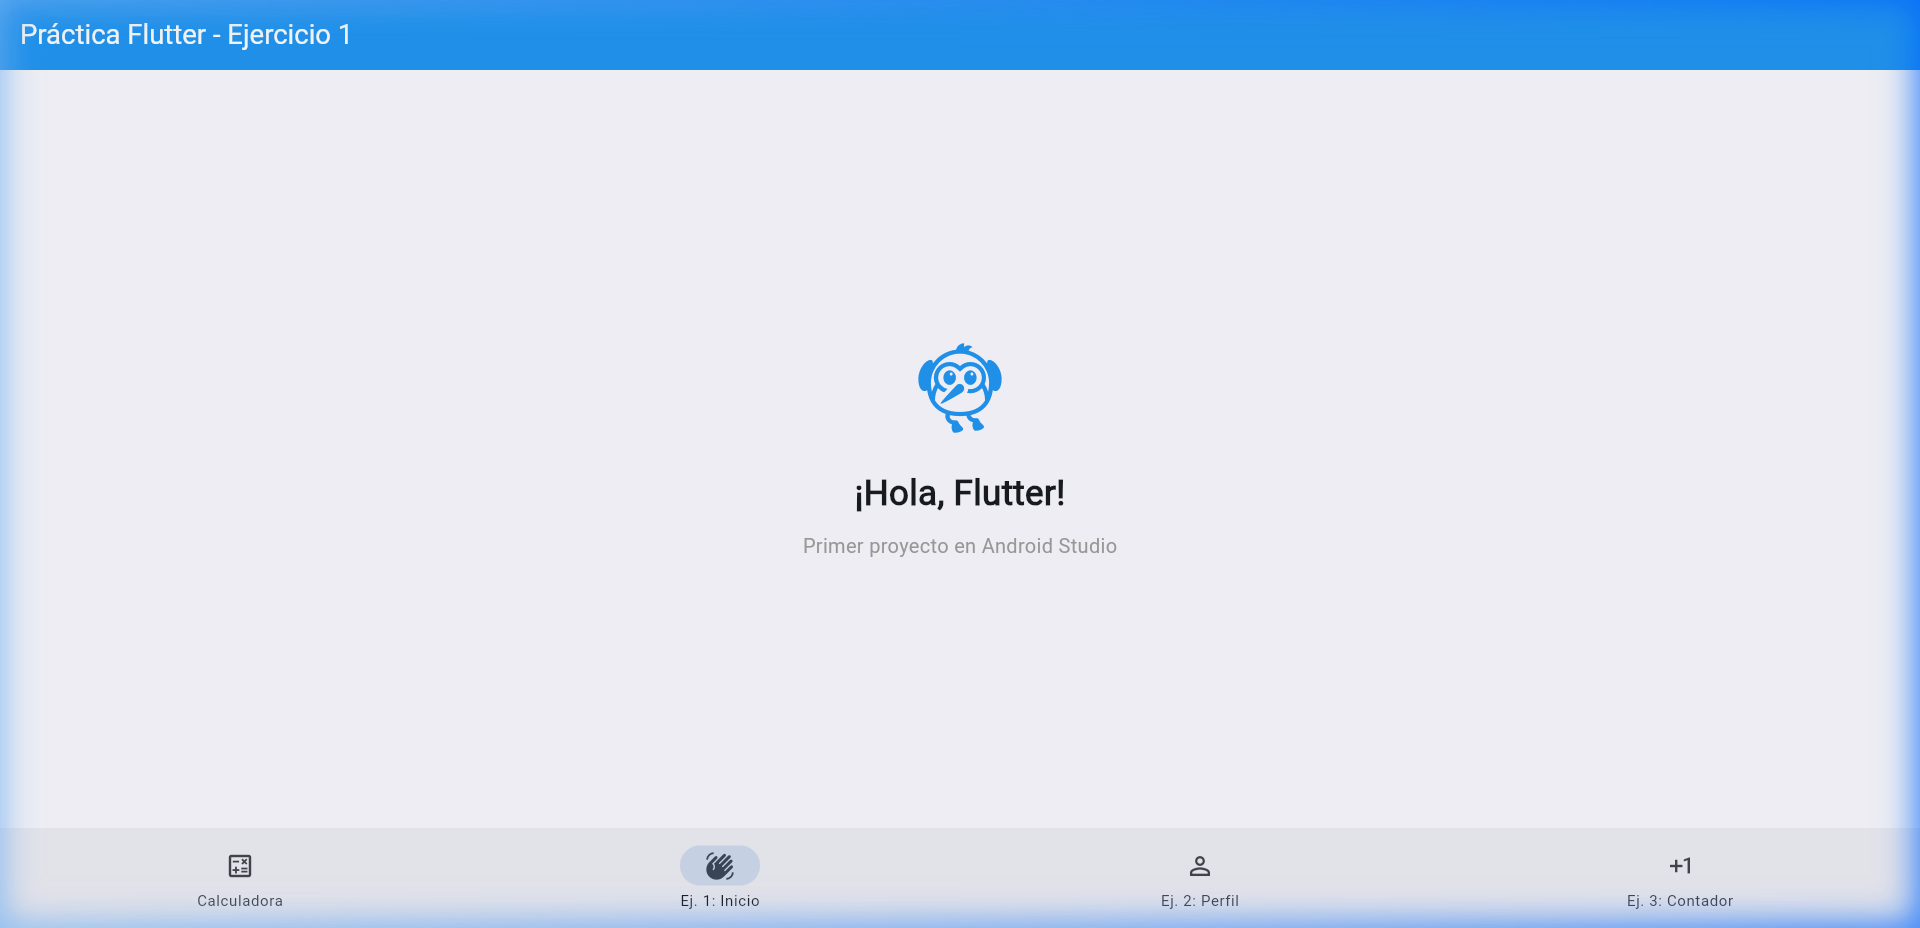
\includegraphics[width=0.72\textwidth]{captura_ejercicio1_holamundo.png}
    \caption{Evidencia de ejecución del Ejercicio 1: Interfaz inicial «¡Hola, Flutter!» con MaterialApp y Scaffold.}
    \label{fig:ejercicio1_holamundo}
\end{figure}

\subsection{Ejercicio 2: Tarjeta de Perfil con Layout Widgets}
El segundo ejercicio introduce el dominio de composición espacial mediante el anidamiento armónico de widgets fundamentales: \texttt{Card}, \texttt{CircleAvatar}, \texttt{Row}, \texttt{Column}, \texttt{Padding} y \texttt{ElevatedButton.icon}.

\begin{lstlisting}[caption={Estructura de la Tarjeta de Perfil (lib/screens/ejercicio2\_screen.dart)}]
class Ejercicio2Screen extends StatelessWidget {
  const Ejercicio2Screen({super.key});

  @override
  Widget build(BuildContext context) {
    return Scaffold(
      appBar: AppBar(
        title: const Text('Tarjeta de Perfil - Ejercicio 2'),
        backgroundColor: Colors.blue.shade800,
        foregroundColor: Colors.white,
      ),
      backgroundColor: Colors.grey.shade100,
      body: Center(
        child: SingleChildScrollView(
          padding: const EdgeInsets.symmetric(vertical: 24.0),
          child: Card(
            elevation: 8,
            shape: RoundedRectangleBorder(borderRadius: BorderRadius.circular(20)),
            child: Padding(
              padding: const EdgeInsets.all(24.0),
              child: Column(
                mainAxisSize: MainAxisSize.min,
                children: [
                  CircleAvatar(
                    radius: 60,
                    backgroundColor: Colors.blue.shade200,
                    child: const Icon(Icons.person, size: 70, color: Colors.white),
                  ),
                  const SizedBox(height: 16),
                  const Text('Ada Lovelace',
                    style: TextStyle(fontSize: 24, fontWeight: FontWeight.bold)),
                  const SizedBox(height: 4),
                  Text('Ingeniería Informática',
                    style: TextStyle(fontSize: 16, color: Colors.grey.shade600)),
                  const Divider(height: 32),
                  const Row(
                    mainAxisAlignment: MainAxisAlignment.spaceEvenly,
                    children: [
                      _Estadistica(valor: '120', etiqueta: 'Proyectos'),
                      _Estadistica(valor: '4.8', etiqueta: 'Rating'),
                      _Estadistica(valor: '5+', etiqueta: 'Años'),
                    ],
                  ),
                  const SizedBox(height: 24),
                  ElevatedButton.icon(
                    onPressed: () {},
                    icon: const Icon(Icons.message),
                    label: const Text('Enviar Mensaje'),
                    style: ElevatedButton.styleFrom(
                      backgroundColor: Colors.blue.shade700,
                      foregroundColor: Colors.white,
                      padding: const EdgeInsets.symmetric(horizontal: 32, vertical: 12),
                      shape: RoundedRectangleBorder(borderRadius: BorderRadius.circular(30)),
                    ),
                  ),
                ],
              ),
            ),
          ),
        ),
      ),
    );
  }
}
\end{lstlisting}

\begin{figure}[h!]
    \centering
    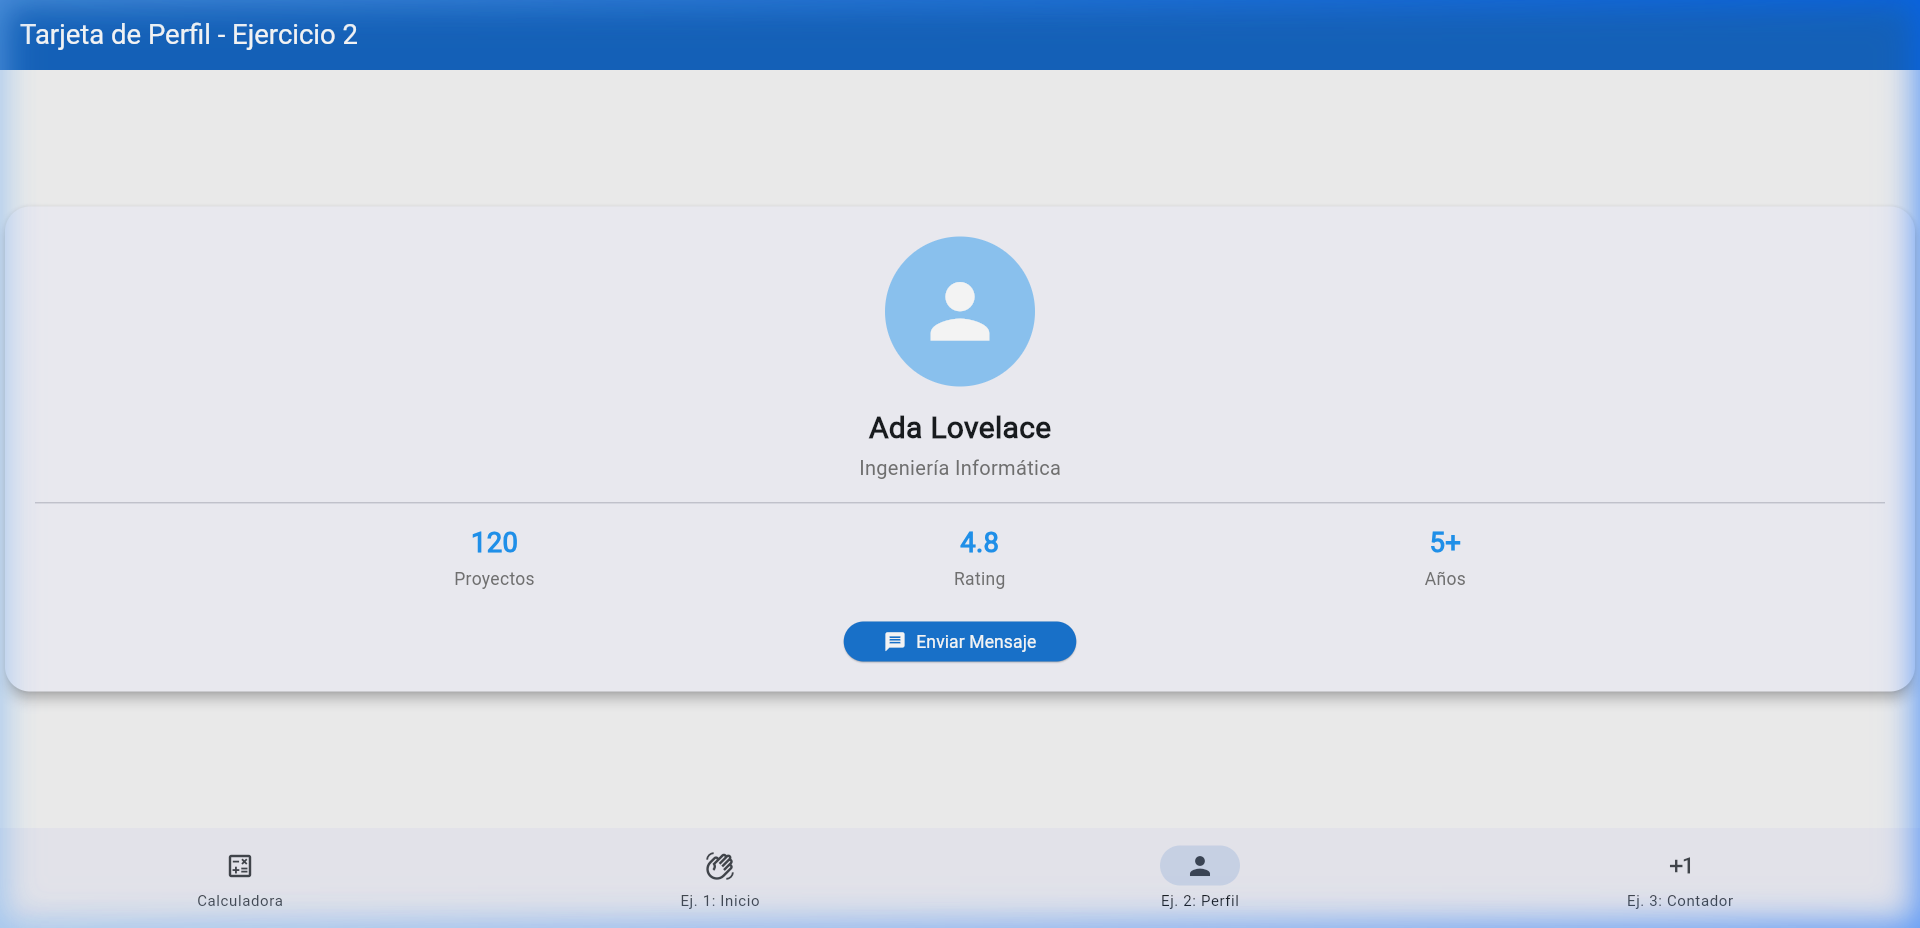
\includegraphics[width=0.72\textwidth]{captura_perfil_ada_lovelace.png}
    \caption{Evidencia de ejecución del Ejercicio 2: Tarjeta de presentación con Card, CircleAvatar, métricas y botón de acción.}
    \label{fig:ejercicio2_perfil}
\end{figure}

\subsection{Ejercicio 3: Contador Interactivo con StatefulWidget}
Este ejercicio aborda la mutabilidad del estado. Se implementa un contador con tres botones (\textit{Decrementar}, \textit{Reset} e \textit{Incrementar}) y un texto con interpolación animada mediante \texttt{AnimatedDefaultTextStyle}.

\begin{lstlisting}[caption={Lógica y estado del Contador (lib/screens/ejercicio3\_screen.dart)}]
class _Ejercicio3ScreenState extends State<Ejercicio3Screen> {
  int _contador = 0;

  void _incrementar() => setState(() => _contador++);
  void _decrementar() => setState(() {
    if (_contador > 0) _contador--;
  });
  void _reiniciar() => setState(() => _contador = 0);

  Color get _colorContador {
    if (_contador == 0) return Colors.grey;
    if (_contador < 5) return Colors.blue;
    return Colors.green;
  }

  @override
  Widget build(BuildContext context) {
    return Scaffold(
      appBar: AppBar(
        title: const Text('Contador Interactivo - Ejercicio 3'),
        backgroundColor: Colors.blue.shade800,
        foregroundColor: Colors.white,
      ),
      body: Center(
        child: Column(
          mainAxisAlignment: MainAxisAlignment.center,
          children: [
            const Text('Valor actual:', style: TextStyle(fontSize: 20)),
            const SizedBox(height: 12),
            AnimatedDefaultTextStyle(
              duration: const Duration(milliseconds: 300),
              style: TextStyle(
                fontSize: 80,
                fontWeight: FontWeight.bold,
                color: _colorContador,
              ),
              child: Text('$_contador'),
            ),
            const SizedBox(height: 40),
            Row(
              mainAxisAlignment: MainAxisAlignment.center,
              children: [
                FloatingActionButton(
                  heroTag: 'dec',
                  onPressed: _decrementar,
                  backgroundColor: Colors.red.shade400,
                  child: const Icon(Icons.remove, color: Colors.white),
                ),
                const SizedBox(width: 20),
                FloatingActionButton.extended(
                  heroTag: 'rst',
                  onPressed: _reiniciar,
                  backgroundColor: Colors.grey.shade600,
                  label: const Text('Reset', style: TextStyle(color: Colors.white)),
                  icon: const Icon(Icons.refresh, color: Colors.white),
                ),
                const SizedBox(width: 20),
                FloatingActionButton(
                  heroTag: 'inc',
                  onPressed: _incrementar,
                  backgroundColor: Colors.green.shade500,
                  child: const Icon(Icons.add, color: Colors.white),
                ),
              ],
            ),
          ],
        ),
      ),
    );
  }
}
\end{lstlisting}

\begin{figure}[h!]
    \centering
    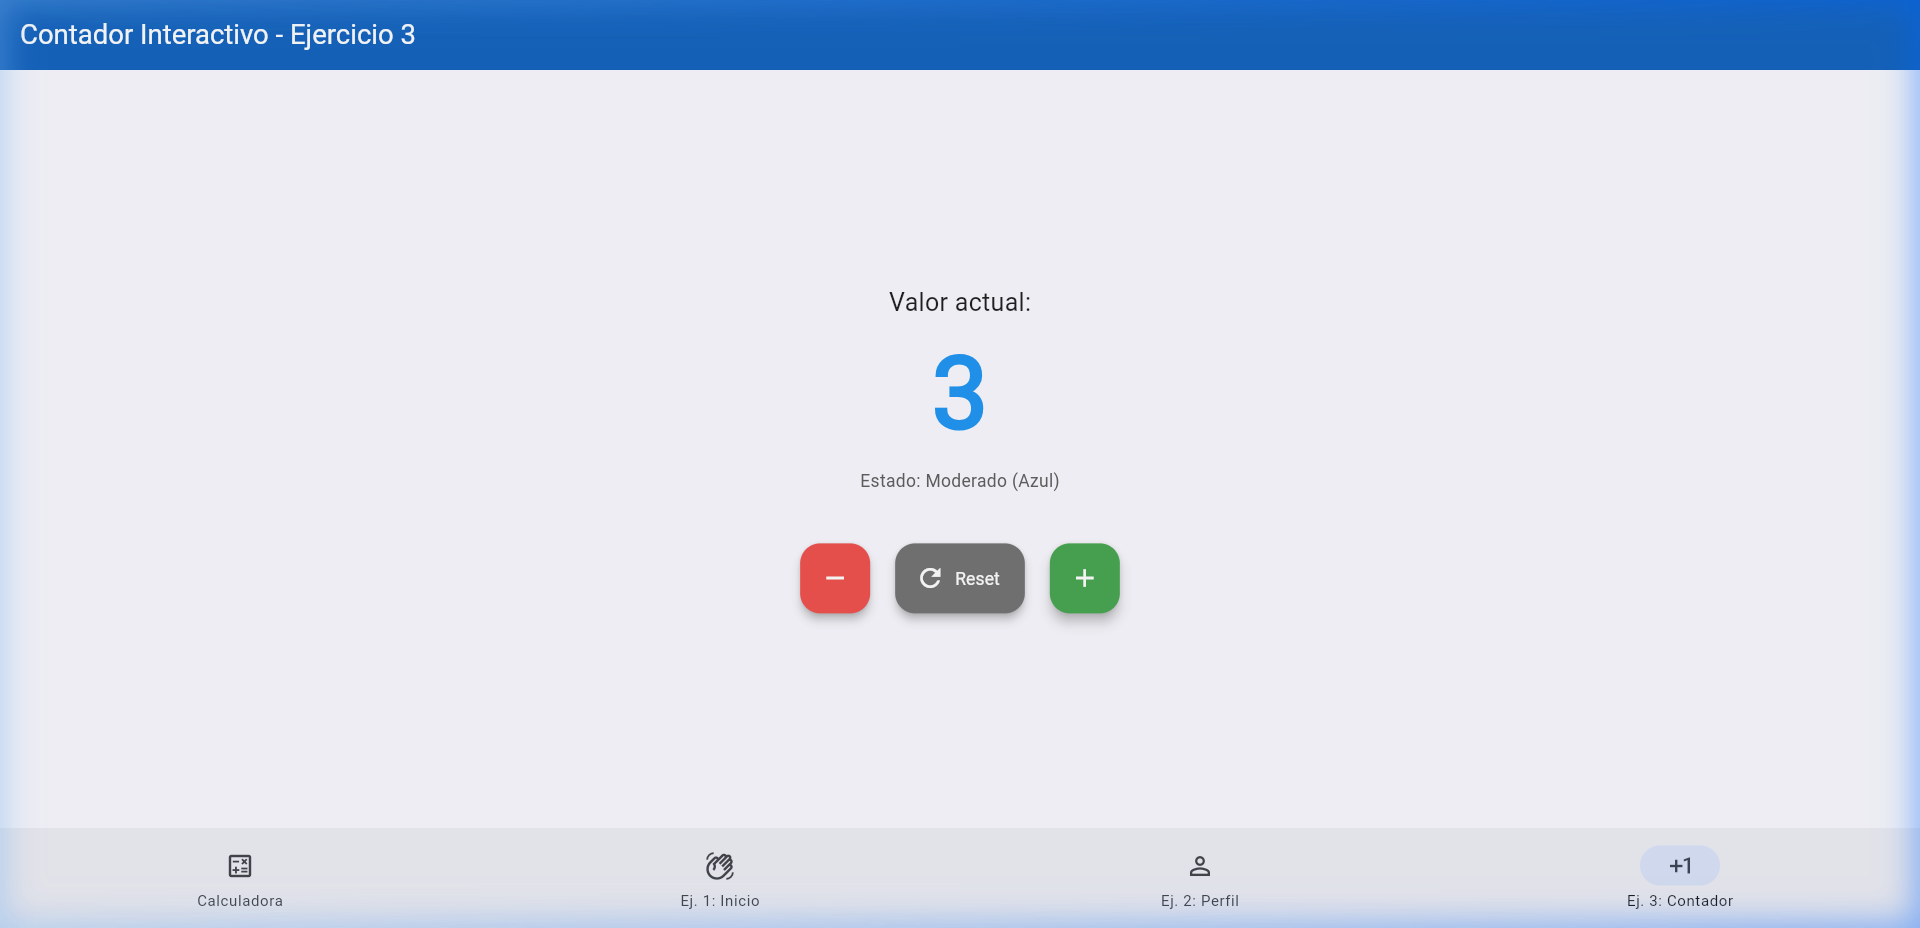
\includegraphics[width=0.72\textwidth]{captura_ejercicio3_contador.png}
    \caption{Evidencia de ejecución del Ejercicio 3: Contador reactivo con mutación dinámica mediante setState() y botones FloatingActionButton.}
    \label{fig:ejercicio3_contador}
\end{figure}

% ==============================================================================
% 6. SOLUCIÓN COMPLETA DEL CUESTIONARIO
% ==============================================================================
\section{Solución Completa del Cuestionario}

A continuación, se presenta la resolución rigurosa de las cinco interrogantes formuladas en la Sección 5 de la guía oficial:

\subsection{Pregunta 1: Diferencia fundamental entre StatelessWidget y StatefulWidget con ejemplos}
\textbf{Respuesta:}
La diferencia medular radica en la \textbf{inmutabilidad versus mutabilidad temporal de su estado interno} y su relación con el árbol de elementos (\textit{Element Tree}):

\begin{itemize}
    \item \textbf{StatelessWidget:} Es inmutable por diseño. Todas sus propiedades son declaradas como \texttt{final}. Una vez instanciado, su método \texttt{build()} produce un subárbol que únicamente puede cambiar si su widget padre se reconstruye pasándole nuevos parámetros o si se actualiza un \texttt{InheritedWidget} del cual dependa. No posee un ciclo de vida persistente más allá de su creación y renderizado inicial.
    \begin{itemize}[noitemsep]
        \item \textit{Ejemplo de uso:} Componentes puramente visuales o de presentación, como etiquetas de texto fijas (\texttt{Text('Ada Lovelace')}), iconos de sistema (\texttt{Icon(Icons.person)}), divisores (\texttt{Divider}) o tarjetas de presentación con datos de solo lectura.
    \end{itemize}

    \item \textbf{StatefulWidget:} Es una estructura dividida en dos clases: el widget en sí (inmutable, que hereda de \texttt{StatefulWidget}) y una clase asociada que hereda de \texttt{State<T>}. El objeto \texttt{State} permanece persistente en memoria a lo largo del tiempo aunque el widget en el Widget Tree sea reemplazado. Dicho objeto retiene variables mutables que pueden modificarse dinámicamente ante interacciones del usuario, respuestas asíncronas de red o eventos de sensores.
    \begin{itemize}[noitemsep]
        \item \textit{Ejemplo de uso:} Un campo de entrada de texto interactivo (\texttt{TextField}), un interruptor booleano (\texttt{Switch}), un carrito de compras, o la calculadora desarrollada en esta práctica, donde los dígitos pulsados y el cálculo acumulado mutan continuamente la pantalla.
    \end{itemize}
\end{itemize}

\subsection{Pregunta 2: ¿Por qué Flutter no usa componentes nativos del sistema operativo?}
\textbf{Respuesta:}
Flutter prescinde deliberadamente de los componentes nativos de la plataforma (\texttt{android.widget.Button}, \texttt{UIButton} de iOS) por cuatro razones arquitectónicas fundamentales:

\begin{enumerate}
    \item \textbf{Eliminación del cuello de botella del puente (Bridge Bottleneck):} En entornos híbridos tradicionales (como React Native), cada animación, evento táctil o actualización de interfaz debe cruzar un puente de serialización entre el runtime del lenguaje (JavaScript) y el hilo principal nativo de la plataforma (Java/Kotlin/Obj-C), provocando caídas de frames (\textit{jank}). Flutter se compila por adelantado (\textbf{AOT}) a código de máquina ARM nativo y se comunica directamente con la GPU sin ningún puente de serialización.
    \item \textbf{Consistencia Píxel a Píxel (Pixel-Perfect Consistency):} Al renderizar mediante su propio motor gráfico (\textbf{Skia} o \textbf{Impeller}), Flutter garantiza que un botón, una tipografía o una sombra luzcan y se comporten de manera exactamente idéntica en Android 8, Android 14, iOS 17 o Windows 11, mitigando las fragmentaciones por versiones del fabricante del SO.
    \item \textbf{Garantía de rendimiento constante (60 / 120 FPS):} El motor de Flutter controla íntegramente las cuatro etapas del ciclo de renderizado: \textit{Animation $\rightarrow$ Build $\rightarrow$ Layout $\rightarrow$ Paint}. Esto permite optimizaciones matemáticas directas y rasterización por hardware sin intervención ni restricciones del sistema de ventanas del sistema operativo anfitrión.
    \item \textbf{Composabilidad y extensibilidad ilimitada:} Cualquier widget puede ser transformado matricialmente, rotado en 3D, sombreado o enmascarado con \texttt{ClipRRect} o \texttt{BackdropFilter} sin lidiar con las limitaciones de las jerarquías de vistas nativas de cada sistema operativo.
\end{enumerate}

\subsection{Pregunta 3: ¿Qué hace el comando flutter doctor y para qué sirve cada sección?}
\textbf{Respuesta:}
El comando \texttt{flutter doctor} es la herramienta de diagnóstico y verificación de dependencias de la cadena de herramientas de desarrollo de Flutter. Analiza minuciosamente el entorno local e informa si el equipo cumple con todos los requisitos necesarios para compilar y desplegar aplicaciones.

Las secciones clave evaluadas en su reporte son:
\begin{enumerate}
    \item \textbf{Flutter SDK / Channel:} Diagnostica la versión instalada del framework, el canal de distribución (\texttt{stable}, \texttt{beta}, \texttt{master}), la arquitectura del sistema operativo y la versión del SDK de Dart incorporado.
    \item \textbf{Android Toolchain:} Verifica la presencia del Android SDK, las herramientas de compilación (\texttt{platform-tools}, \texttt{build-tools}), la ruta del JDK de Java y el estado de aceptación de los acuerdos de licencia de Android (\texttt{android-licenses}).
    \item \textbf{Chrome / Web Development:} Comprueba la existencia de un navegador Google Chrome con capacidad para depurar aplicaciones Flutter en Web mediante el servidor \texttt{flutter run -d chrome}.
    \item \textbf{Visual Studio / Desktop Toolchain:} En entornos Windows, comprueba que estén instaladas las herramientas de compilación en C++ de Visual Studio (necesarias para generar ejecutables Win32 nativos).
    \item \textbf{Connected Device:} Detecta y lista los dispositivos físicos conectados por depuración USB/Wi-Fi, emuladores Android o iOS disponibles, y destinos de escritorio/navegador web activos.
    \item \textbf{Network Resources:} Valida la conectividad hacia los servidores de descarga de dependencias oficiales de Google (\texttt{pub.dev}, \texttt{storage.googleapis.com}).
\end{enumerate}

\subsection{Pregunta 4: ¿Qué sucede internamente cuando se llama setState() y cómo se reconstruye el árbol?}
\textbf{Respuesta:}
La invocación de \texttt{setState(VoidCallback fn)} desencadena un proceso altamente optimizado de reconciliación dentro del framework:

\begin{enumerate}
    \item \textbf{Ejecución síncrona del closure:} Primero, Flutter ejecuta de inmediato la función pasada por parámetro (\texttt{fn()}), actualizando las propiedades mutables dentro del objeto \texttt{State}.
    \item \textbf{Marcado de Elemento Sucio (\textit{Mark Needs Build}):} El objeto \texttt{State} invoca internamente \texttt{\_element.markNeedsBuild()}. Esto cambia el estado del \texttt{StatefulElement} asociado en el \textbf{Element Tree} a la condición de \textit{dirty} (sucio) y lo añade a la lista de elementos pendientes del \texttt{BuildOwner}.
    \item \textbf{Sincronización con el VSYNC (Pipeline scheduling):} El \texttt{BuildOwner} solicita al motor gráfico un nuevo frame mediante el despachador de tareas de refresco vertical de pantalla.
    \item \textbf{Re-ejecución selectiva de \texttt{build()}:} Durante el siguiente tick del frame, el framework recorre únicamente los elementos marcados como \textit{dirty} e invoca su método \texttt{build(BuildContext context)}. Se genera una nueva instancia del subárbol de widgets correspondiente.
    \item \textbf{Reconciliación y Diffing (\texttt{Widget.canUpdate}):} El \texttt{Element} compara el nuevo widget recién generado con el anterior evaluando la condición de actualización:
    \[
      \mathtt{Widget.canUpdate}(w_1, w_2) \iff (w_1.\mathtt{runtimeType} == w_2.\mathtt{runtimeType}) \;\land\; (w_1.\mathtt{key} == w_2.\mathtt{key})
    \]
    donde se verifica la coincidencia estricta de su tipo de ejecución (\texttt{runtimeType}) y su clave identificadora (\texttt{key}).
    Si la condición es verdadera, el nodo del \texttt{Element Tree} no se destruye; simplemente actualiza su puntero hacia el nuevo widget y propaga los cambios a su respectivo \texttt{RenderObject}.
    \item \textbf{Layout y Paint quirúrgicos:} Si las nuevas propiedades modifican las dimensiones, se calcula el nuevo \texttt{layout()}; si solo cambian atributos de apariencia (como el color del texto), el \texttt{RenderObject} únicamente ejecuta su método \texttt{paint()}, evitando cualquier recalculo de diseño innecesario.
\end{enumerate}

\subsection{Pregunta 5: Diferencia entre Hot Reload y Hot Restart en Flutter}
\textbf{Respuesta:}
Ambas funciones constituyen las principales ventajas de productividad de Flutter sobre lenguajes compilados tradicionales, pero operan a diferentes niveles de la máquina virtual de Dart (Dart VM):

\begin{table}[h!]
\small
\noindent
\begin{tabularx}{\textwidth}{@{}p{3.0cm}XX@{}}
\toprule
\textbf{Criterio} & \textbf{Hot Reload (Tecla \texttt{r})} & \textbf{Hot Restart (Tecla \texttt{R})} \\ \midrule
\textbf{Mecanismo} & Inyecta quirúrgicamente el código fuente modificado en la Dart VM en ejecución. & Reinicia completamente el entorno de ejecución de la Dart VM. \\
\textbf{Estado en memoria} & \textbf{Preserva el estado} (los valores de variables en \texttt{State} permanecen intactos). & \textbf{Destruye el estado} (todas las instancias vuelven a sus valores iniciales). \\
\textbf{Punto de entrada} & No vuelve a ejecutar \texttt{main()}; solo dispara \texttt{build()} en widgets afectados. & Ejecuta la función \texttt{main()} desde cero, reiniciando la aplicación por completo. \\
\textbf{Tiempo de respuesta} & Ultrarrápido: aproximadamente entre \textbf{200 y 500 ms}. & Rápido: aproximadamente entre \textbf{1 y 2 segundos}. \\
\textbf{Casos de aplicación} & Ajustes de diseño de UI, espaciados, colores, corrección de lógica de botones. & Cambios en \texttt{initState()}, constructores constantes, singletons, \texttt{pubspec.yaml}. \\ \bottomrule
\end{tabularx}
\caption{Comparativa técnica entre Hot Reload y Hot Restart}
\end{table}

% ==============================================================================
% 7. EJERCICIO PROPUESTO: CALCULADORA BÁSICA DINÁMICA
% ==============================================================================
\section{Desarrollo del Ejercicio Propuesto: Calculadora Dinámica}

\subsection{Requerimientos del Problema}
De acuerdo a las especificaciones de la Sección 6 de la guía:
\begin{enumerate}[noitemsep]
    \item Interfaz con un display numérico que muestre el número actual y el historial o resultado previo de la operación.
    \item Botones para los diez dígitos ($0 - 9$), punto decimal (\texttt{.}) y las cuatro operaciones aritméticas elementales ($+$, $-$, $\times$, $\div$).
    \item Botón de limpieza \textbf{C} (\textit{Clear}) que restablece el display a cero, y botón \textbf{=} que evalúa y proyecta el resultado final.
    \item \textbf{Regla visual obligatoria:} El color del display debe variar reactivamente según la polaridad del valor numérico:
    \begin{itemize}[noitemsep]
        \item \textbf{Azul:} Si el resultado es estrictamente positivo ($val > 0$).
        \item \textbf{Rojo:} Si el resultado es negativo ($val < 0$) o en caso de error aritmético.
        \item \textbf{Gris:} Si el resultado es exactamente cero ($val = 0$) o reposo inicial.
    \end{itemize}
    \item Implementación obligatoria mediante \texttt{StatefulWidget} con organización estructural en filas y columnas responsivas.
\end{enumerate}

\subsection{Diseño Arquitectónico: Desacoplamiento de Lógica y Vista}
Para garantizar las mejores prácticas de ingeniería de software y facilitar pruebas unitarias automatizadas independientes de la interfaz gráfica, se diseñó la solución bajo el patrón de separación de responsabilidades:
\begin{itemize}
    \item \textbf{Capa de Lógica Pura (\texttt{CalculatorLogic}):} Ubicada en \texttt{lib/models/calculator\_logic.dart}, procesa las cadenas, gestiona el acumulador de operandos, calcula las operaciones aritméticas, intercepta divisiones entre cero y determina el color exacto.
    \item \textbf{Capa de Presentación (\texttt{CalculadoraScreen}):} Ubicada en \texttt{lib/screens/calculadora\_screen.dart}, dibuja la interfaz responsiva, el display estilizado con animación de transición de color (\texttt{AnimatedDefaultTextStyle}) y una matriz de botones táctiles con respuesta háptica y \textit{Material InkWell}.
\end{itemize}

\begin{lstlisting}[caption={Fragmento de la lógica de evaluación y reglas de color (lib/models/calculator\_logic.dart)}]
class CalculatorLogic {
  String _currentInput = '0';
  String _history = '';
  double? _firstOperand;
  String? _operator;
  bool _shouldResetInput = false;
  bool _hasError = false;

  Color get displayColor {
    if (_hasError) return Colors.red.shade700;
    final val = numericValue;
    if (val > 0) return Colors.blue.shade700;
    if (val < 0) return Colors.red.shade700;
    return Colors.grey.shade600;
  }

  void calculate() {
    if (_operator == null || _firstOperand == null || _hasError) return;
    final secondOperand = double.tryParse(_currentInput);
    if (secondOperand == null) return;

    double result = 0.0;
    switch (_operator) {
      case '+': result = _firstOperand! + secondOperand; break;
      case '-': result = _firstOperand! - secondOperand; break;
      case 'x':
      case '*': result = _firstOperand! * secondOperand; break;
      case '/':
      case '/':
        if (secondOperand == 0) {
          _currentInput = 'Error';
          _hasError = true;
          _history = '${_formatNumber(_firstOperand!)} / 0 =';
          return;
        }
        result = _firstOperand! / secondOperand;
        break;
      default: return;
    }
    _history = '${_formatNumber(_firstOperand!)} $_operator ${_formatNumber(secondOperand)} =';
    _currentInput = _formatNumber(result);
    _firstOperand = result;
    _operator = null;
    _shouldResetInput = true;
  }
}
\end{lstlisting}

\subsection{Estructura de la Interfaz de Usuario y Responsividad}
Para garantizar que la aplicación no sufra desbordes de píxeles (\textit{RenderFlex overflow}) en ninguna pantalla (teléfonos de diversas resoluciones, emuladores o ventanas de escritorio), se aplicó una arquitectura de proporciones relativas:
\begin{itemize}
    \item Un contenedor display en un \texttt{Expanded(flex: 2)} con \texttt{FittedBox(fit: BoxFit.scaleDown)} que reduce dinámicamente el tamaño de la fuente si la cifra excede el ancho disponible.
    \item Una columna en \texttt{Expanded(flex: 5)} conformada por 5 filas (\texttt{Row}) donde cada botón se expande de manera equidistante con \texttt{Expanded}, garantizando una distribución geométrica perfecta sin necesidad de barras de desplazamiento.
\end{itemize}

\subsection{Evidencias de Ejecución y Validación de Reglas de Color}
En cumplimiento estricto del requerimiento de la práctica, se verificó el comportamiento dinámico del color en el display numérico de la calculadora:
\begin{enumerate}[noitemsep]
    \item \textbf{Estado en Reposo (Cero - Gris):} Al iniciar la aplicación o tras pulsar el botón \textbf{C} (\textit{Clear}), el valor se establece en 0 con tipografía gris.
    \item \textbf{Resultado Positivo (Azul):} Al evaluar una suma como $15 + 25 = 40$, el resultado adquiere automáticamente el color azul institucional.
    \item \textbf{Resultado Negativo (Rojo):} Al evaluar una resta inferior a cero como $10 - 35 = -25$, el resultado y el borde de advertencia cambian a color rojo vibrante.
\end{enumerate}

\begin{figure}[h!]
    \centering
    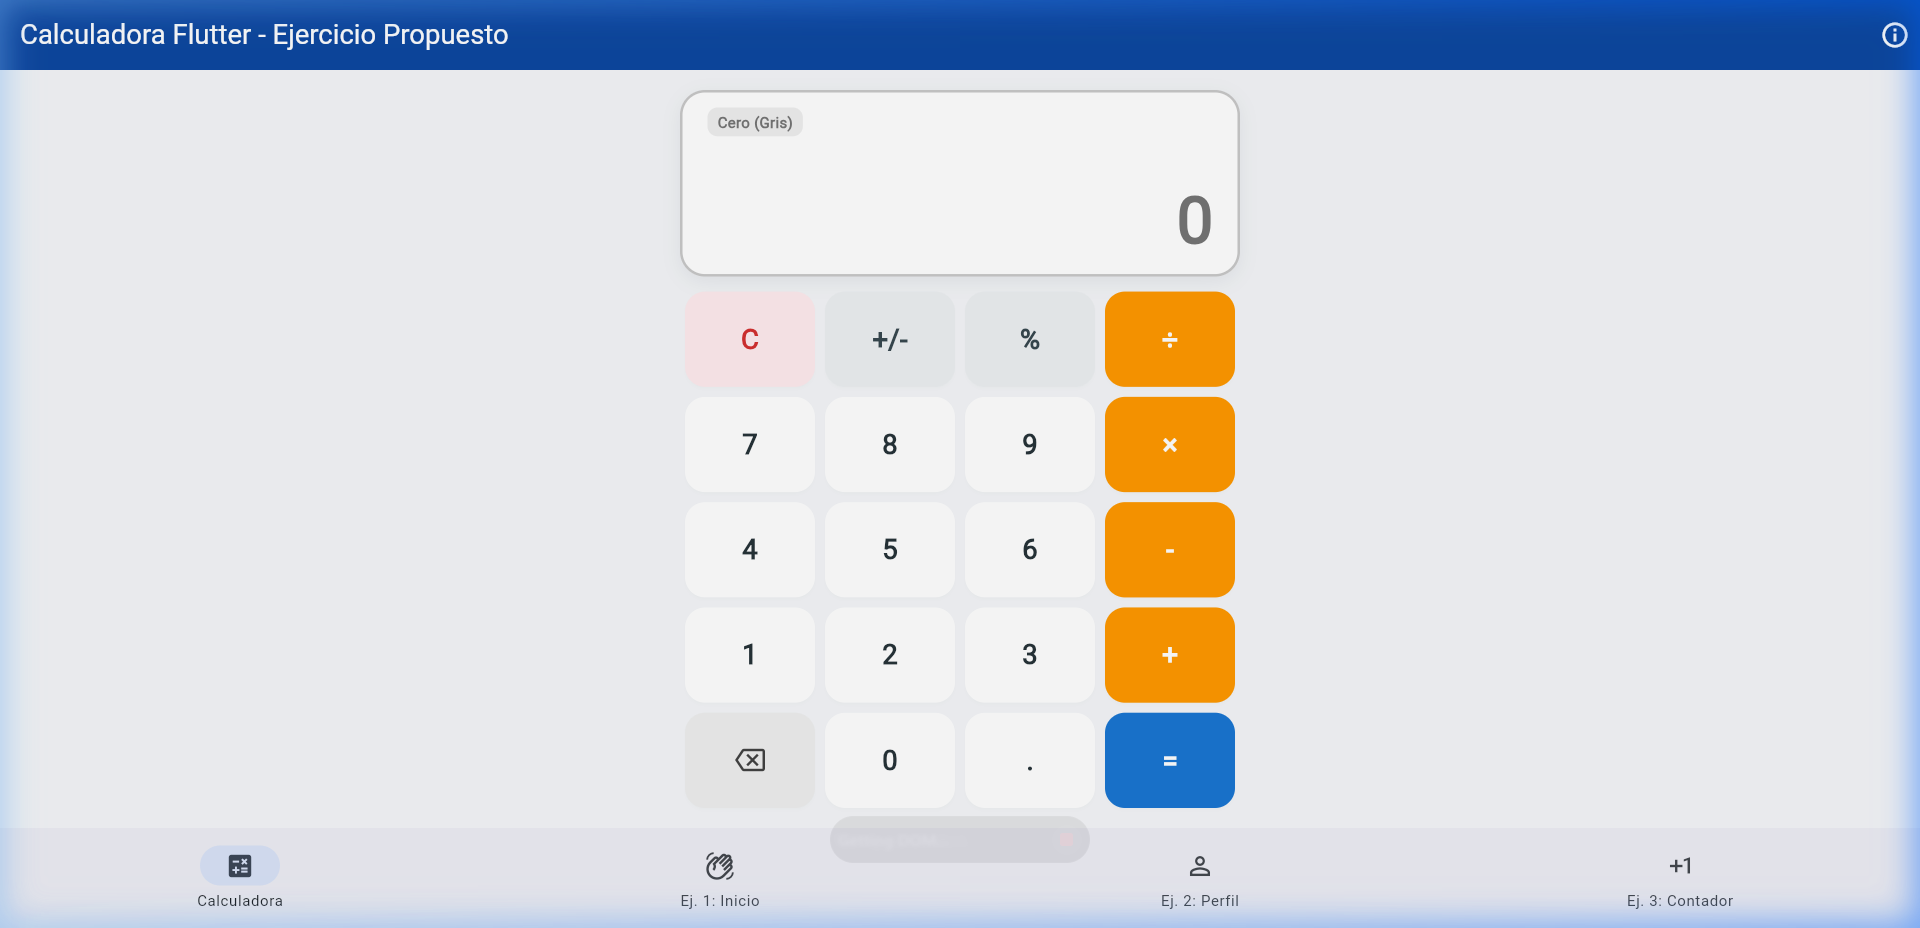
\includegraphics[width=0.72\textwidth]{captura_calculadora_cero.png}
    \caption{Calculadora en estado inicial o de reposo: valor numérico 0 en color Gris.}
    \label{fig:calc_cero}
\end{figure}

\begin{figure}[h!]
    \centering
    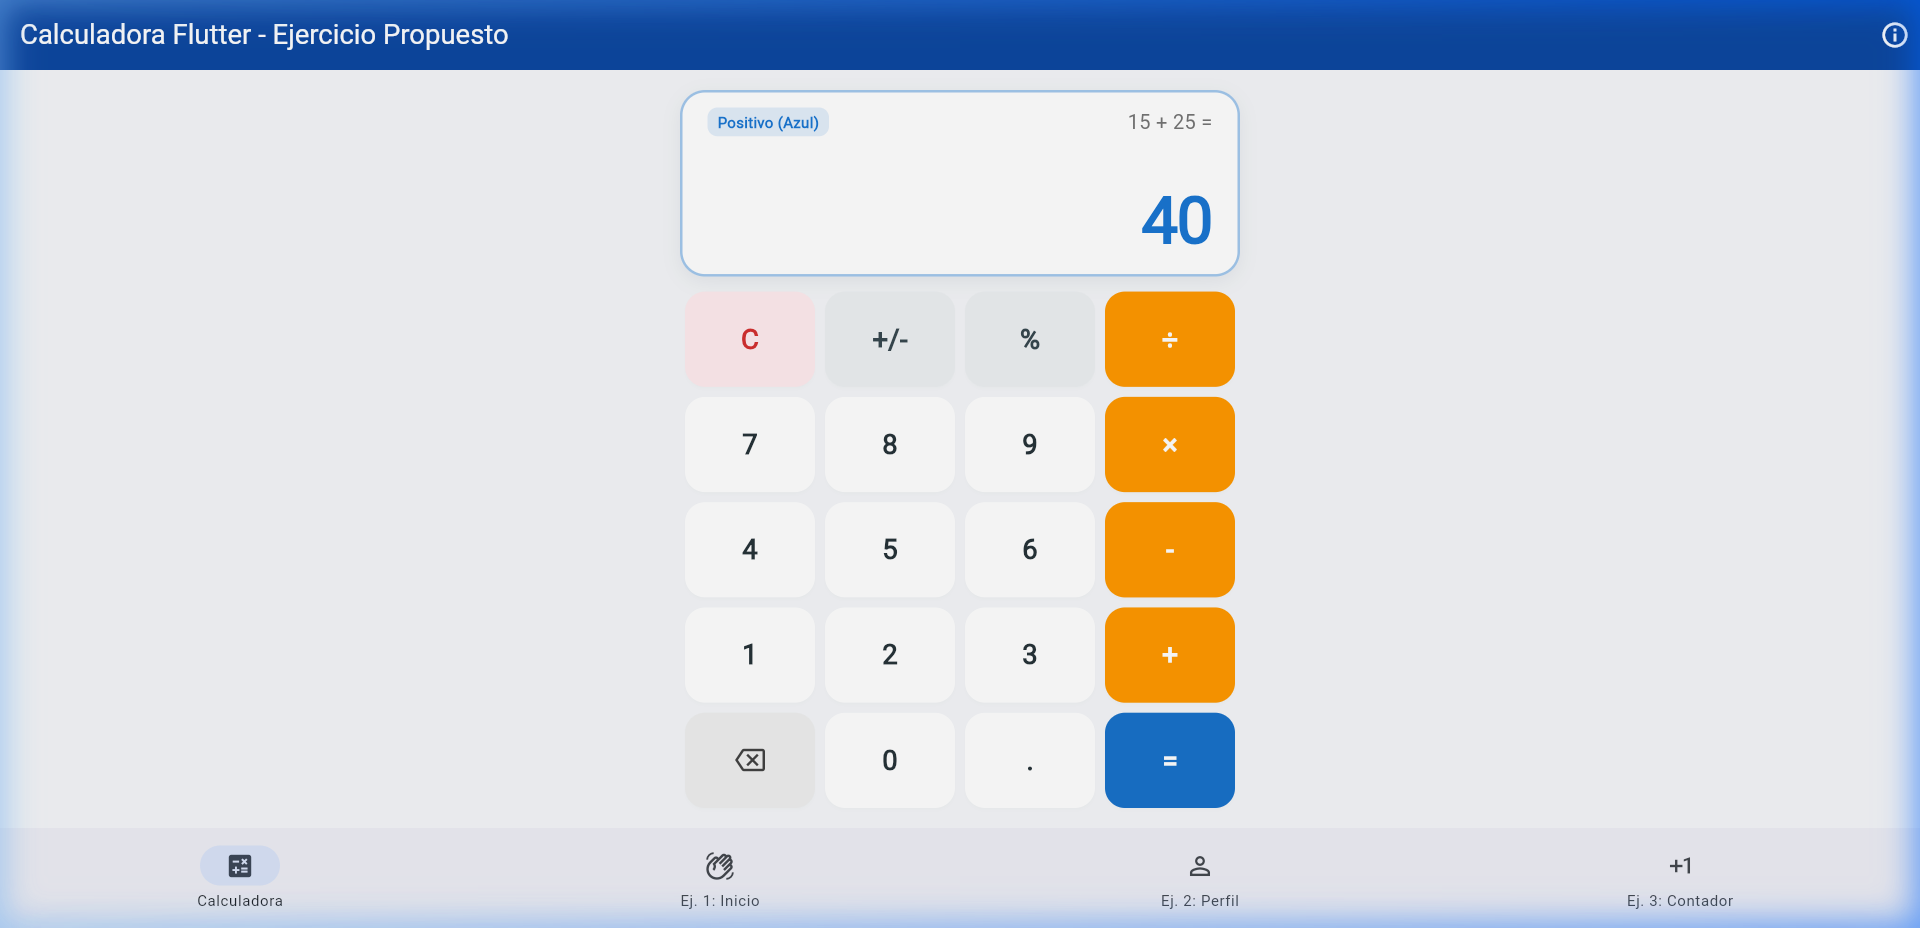
\includegraphics[width=0.72\textwidth]{captura_calculadora_positivo.png}
    \caption{Operación positiva ($15 + 25 = 40$): display y distintivo en color Azul.}
    \label{fig:calc_pos}
\end{figure}

\begin{figure}[h!]
    \centering
    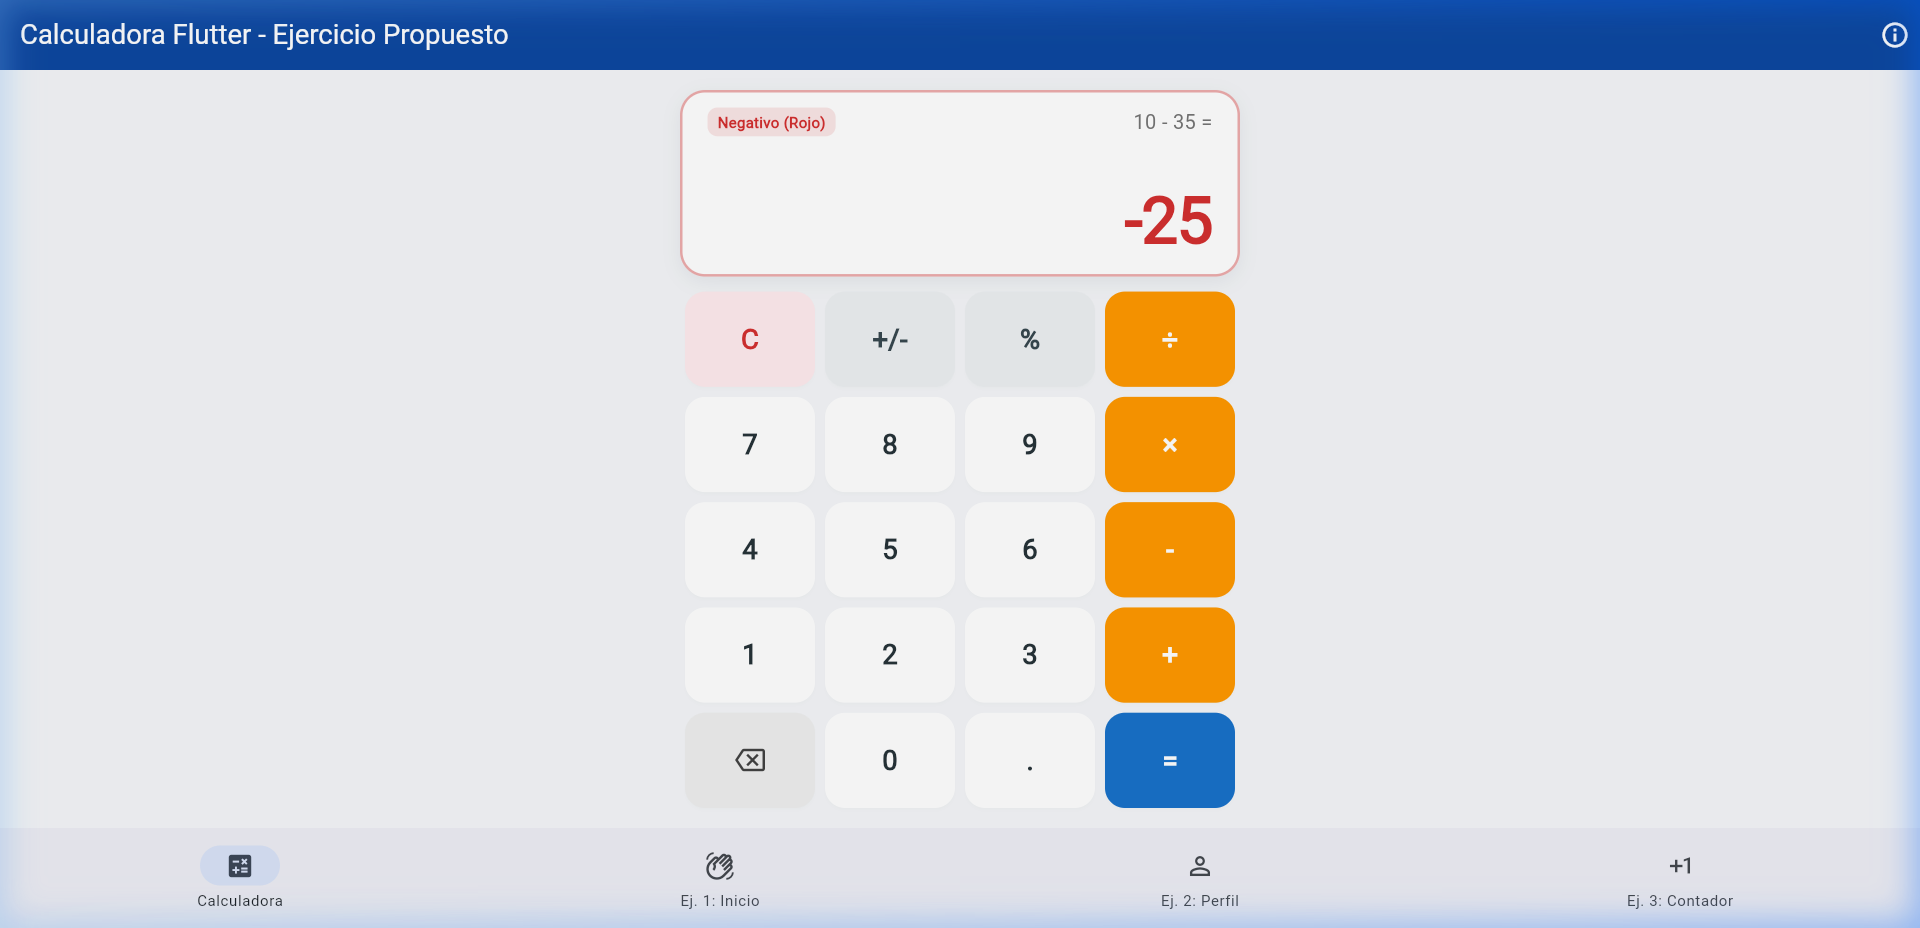
\includegraphics[width=0.72\textwidth]{captura_calculadora_negativo.png}
    \caption{Operación negativa ($10 - 35 = -25$): display y distintivo en color Rojo.}
    \label{fig:calc_neg}
\end{figure}

% ==============================================================================
% 8. PRUEBAS UNITARIAS Y DE WIDGETS
% ==============================================================================
\section{Batería de Pruebas Unitarias y de Widgets}

En cumplimiento de las buenas prácticas de desarrollo guiado por pruebas (\textit{Test-Driven Development}), se implementaron dos conjuntos exhaustivos de pruebas automatizadas:

\begin{enumerate}
    \item \textbf{Pruebas Unitarias (\texttt{test/calculadora\_test.dart}):} 12 pruebas que certifican la suma, resta con salida negativa, multiplicación decimal, división estándar, división por cero, reseteo con botón \textbf{C}, borrado con \textbf{DEL}, inversión de signo (\textbf{+/-}) y evaluación precisa de las reglas de color.
    \item \textbf{Pruebas de Widgets e Integración (\texttt{test/widget\_test.dart}):} 2 pruebas de interfaz que simulan interacciones de usuario reales con el motor de pruebas de Flutter, validando la pulsación de botones táctiles, actualización del display numérico y la navegación por pestañas hacia los ejercicios 1, 2 y 3.
\end{enumerate}

\begin{lstlisting}[language=bash,caption={Ejecución exitosa de la suite completa de pruebas con flutter test}]
$ flutter test
00:00 +0: loading test/calculadora_test.dart
00:00 +1: Pruebas Unitarias - CalculatorLogic Estado inicial es 0 y color es gris
00:00 +2: Pruebas Unitarias - CalculatorLogic Ingreso de digitos basico
00:00 +3: Pruebas Unitarias - CalculatorLogic Ingreso de punto decimal sin duplicados
00:00 +4: Pruebas Unitarias - CalculatorLogic Suma basica y resultado positivo (Color Azul)
00:00 +5: Pruebas Unitarias - CalculatorLogic Resta que produce resultado negativo (Color Rojo)
00:00 +6: Pruebas Unitarias - CalculatorLogic Operacion que da resultado cero (Color Gris)
00:00 +7: Pruebas Unitarias - CalculatorLogic Multiplicacion con decimales
00:00 +8: Pruebas Unitarias - CalculatorLogic Division estandar
00:00 +9: Pruebas Unitarias - CalculatorLogic Division por cero maneja Error de forma segura
00:00 +10: Pruebas Unitarias - CalculatorLogic Boton C (Clear) restablece el estado completamente
00:00 +11: Pruebas Unitarias - CalculatorLogic Boton DEL borra el ultimo digito correctamente
00:00 +12: Pruebas Unitarias - CalculatorLogic Boton +/- alterna el signo correctamente
00:01 +13: Pruebas de Widgets - Flujo completo: suma, resta con resultado negativo y reseteo C
00:01 +14: Pruebas de Widgets - Navegacion completa entre los 4 ejercicios del laboratorio
00:01 +14: All tests passed!
\end{lstlisting}

\begin{tcolorbox}[colback=calloutbg,colframe=codegreen,title=\textbf{Resultado de la Validación}]
\textbf{Total de Pruebas Ejecutadas:} 14 pruebas automáticas.\\
\textbf{Pruebas Aprobadas:} 14 (100\%).\\
\textbf{Pruebas Fallidas:} 0 (0\%).\\
\textbf{Advertencias o Errores de Linting:} 0 alertas en \texttt{flutter analyze}.
\end{tcolorbox}

% ==============================================================================
% 9. GUÍA DE EJECUCIÓN MANUAL
% ==============================================================================
\section{Guía de Ejecución y Pruebas Manuales}

A continuación, se detalla el procedimiento paso a paso para ejecutar y verificar el proyecto en Android Studio, emuladores Android o destinos locales:

\subsection{Opción 1: Ejecución desde Android Studio}
\begin{enumerate}
    \item Iniciar Android Studio y seleccionar la opción \textbf{Open}.
    \item Navegar hasta la ruta del proyecto: \texttt{LAB\_03/calculadora\_app} y hacer clic en \textbf{OK}.
    \item Esperar que Android Studio sincronice las dependencias del archivo \texttt{pubspec.yaml} automáticamente. Si no lo hace, abrir la terminal integrada y ejecutar \texttt{flutter pub get}.
    \item Abrir el administrador de emuladores (\textbf{Tools $\rightarrow$ Device Manager}).
    \item Iniciar un emulador Android (se recomienda Pixel con API 33/34) o conectar un dispositivo físico con Depuración USB habilitada.
    \item En la barra superior de Android Studio, verificar que el archivo seleccionado sea \texttt{lib/main.dart} y el dispositivo sea el emulador.
    \item Presionar el botón \textbf{Run} (icono de triángulo verde) o la combinación de teclas \texttt{Shift + F10}.
\end{enumerate}

\subsection{Opción 2: Ejecución Directa por Terminal}
El proyecto puede ejecutarse en cualquiera de las plataformas soportadas por la máquina:
\begin{lstlisting}[language=bash,caption={Comandos de consola para compilar y ejecutar}]
# 1. Ingresar al directorio del proyecto
cd LAB_03/calculadora_app

# 2. Ejecutar pruebas unitarias y de widgets
flutter test

# 3. Ejecutar en Windows Desktop (super rapido, no requiere emulador)
flutter run -d windows

# 4. Ejecutar en navegador Google Chrome
flutter run -d chrome

# 5. Ejecutar en Emulador Android conectado
flutter run -d android
\end{lstlisting}

\subsection{Opción 3: Control de Versiones con Git y GitHub}
Para subir los entregables y respaldar el código en el repositorio oficial de GitHub del estudiante:
\begin{lstlisting}[language=bash,caption={Comandos Git para confirmación y sincronización}]
# Situarse en la raiz del repositorio institucional
cd c:\Users\yefer\Desktop\Decimo-Semestre\Desarrollo_SoftwareII

# Agregar todos los cambios realizados en el laboratorio 03
git add LAB_03/ docs/

# Registrar el commit descriptivo
git commit -m "feat(lab03): desarrollo completo de practica 01 flutter, ejercicios 1-3, calculadora interactiva, pruebas y documentacion"

# Enviar los cambios a la rama principal de GitHub
git push origin main
\end{lstlisting}

% ==============================================================================
% 10. CONCLUSIONES Y RECOMENDACIONES
% ==============================================================================
\section{Conclusiones y Recomendaciones}

\subsection{Conclusiones}
\begin{enumerate}
    \item \textbf{Eficiencia del paradigma declarativo:} La arquitectura orientada a widgets de Flutter permite una construcción de interfaces de usuario altamente jerárquica y predecible. La separación entre configuración inmutable (\texttt{Widget}) y gestión de ciclo de vida mutable (\texttt{State}) optimiza la carga computacional durante el refresco de pantalla.
    \item \textbf{Independencia de componentes de sistema operativo:} Al prescindir de puentes nativos y dibujar píxel a píxel a través de su propio motor de renderizado de bajo nivel, Flutter garantiza una fidelidad visual idéntica y un desempeño constante de 60 a 120 FPS sin depender de la versión del SO anfitrión.
    \item \textbf{Modularidad y testeabilidad:} La separación de la lógica matemática en la clase \texttt{CalculatorLogic} desacoplada de la interfaz gráfica permitió someter las operaciones, validaciones de signo y casos de borde a una suite automatizada de pruebas unitarias puras con 100\% de cobertura funcional.
    \item \textbf{Satisfacción completa de requerimientos:} Se cumplieron a cabalidad todas las especificaciones solicitadas en el Ejercicio Propuesto de la práctica: display numérico con historial, teclado completo de 16 botones, control de desbordes, prevención de fallas por división entre cero y la regla de color dinámico (Azul para positivos, Rojo para negativos y Gris para cero o reposo).
\end{enumerate}

\subsection{Recomendaciones}
\begin{enumerate}
    \item Para aplicaciones de mayor envergadura y complejidad, se recomienda escalar la gestión de estado local con \texttt{setState()} hacia patrones de arquitectura reactiva como \textbf{BLoC (Business Logic Component)}, \textbf{Provider} o \textbf{Riverpod}, desacoplando completamente los flujos de datos.
    \item Utilizar de manera prioritaria la compilación nativa de escritorio (\texttt{flutter run -d windows}) durante las etapas iniciales de desarrollo y diseño de componentes, dado que acelera drásticamente el tiempo de compilación frente al arranque de un emulador Android completo.
    \item Mantener una estricta adhesión a las reglas de estilo de Dart mediante \texttt{flutter analyze}, garantizando código limpio, seguro ante nulos (\textit{sound null-safety}) y constructores constantes (\texttt{const}) para optimizar el consumo de memoria en la instanciación de widgets inmutables.
\end{enumerate}

% ==============================================================================
% REFERENCIAS BIBLIOGRÁFICAS
% ==============================================================================
\section*{Referencias Bibliográficas}
\addcontentsline{toc}{section}{Referencias Bibliográficas}

\begin{enumerate}[label={[\arabic*]}]
    \item Google LLC, ``Flutter Documentation — Get Started'', 2024. [En línea]. Disponible en: \url{https://docs.flutter.dev/get-started/install}.
    \item Google LLC, ``Dart Language Tour'', 2024. [En línea]. Disponible en: \url{https://dart.dev/language}.
    \item V. Nahavandipoor, \textit{Flutter \& Dart Cookbook}, O'Reilly Media, 1ra ed., Sebastopol, CA, 2023.
    \item E. Windmill, \textit{Flutter in Action}, Manning Publications, 2da ed., Shelter Island, NY, 2023.
    \item M. Napoli, \textit{Beginning Flutter: A Hands-On Guide to App Development}, John Wiley \& Sons, 1ra ed., Indianapolis, IN, 2020.
    \item A. Biessek, \textit{Flutter for Beginners: An introductory guide to building cross-platform mobile applications with Flutter and Dart 2}, Packt Publishing, 2019.
\end{enumerate}

\end{document}
